% Requires: \usepackage{booktabs,graphicx,float}
\section{Large-scale liquidity-shock experiment}
\label{sec:liquidity-shock-experiment}

\subsection{Purpose and design}

This chapter evaluates one experiment from two complementary perspectives.
The computational analysis measures the cost of executing the same coupled
market realisation at different MPI rank counts.  The financial analysis uses
paired shock and no-shock paths to estimate whether a common inventory
constraint transmits a local liquidity disturbance to unshocked books.  The
two analyses therefore share the model, empirical inputs, intervention and
logical event stream; they are separate reports of the same experiment rather
than independent scaling and case studies.

The frozen universe contains 1,480 NASDAQ books from the 30 January 2020
development-validation session.  Symbol-specific background order flow is
combined with ten cluster-level behavioural policies.  The regular session is
represented by 23,400 one-second decision windows.  A fixed, stratified mask
selects 10\% of the books across all ten liquidity clusters.  At
$t^\star=11{,}700$ seconds, an aggressive order equal to three times the
held-out opening best-bid depth is submitted to every selected book.  Its side
is chosen to worsen the shared dealer's pre-shock inventory: a buy when the
dealer is short and a sell otherwise.  This reference dose and direction are
fixed before the counterfactual treatments; the exact asset-level dose vector
must be identical across mechanisms.

The financial design contains three market-maker specifications: a shared
dealer subject to a single global capacity, the same quoting policy with
capacity applied independently to each book, and a control in which the shared
dealer is absent.  Global capacity is evaluated at 800 and 1,600 units per
asset.  Quote size and local capacity are scaled by each symbol's empirical
quote-size proxy, normalised to preserve the declared aggregate capacity.
The uncoupled specification applies the same capacity function separately to
each book; it is not an unlimited-risk dealer.  Shock and no-shock paths use
common random numbers, and each treatment is repeated for 20 seeds.
The empirical adequacy assessment remains bound to the validated
ordinary-market executable.  The corrected shared dealer is introduced only
as a post-validation counterfactual treatment; its manifest records both
executable hashes and explicitly does not extend the empirical validation
claim to the dealer.  Rank equivalence and the mechanism preflight provide
separate implementation evidence for this treatment.

\subsection{Shared-dealer intervention}

Let $q_a(t)$ be the shared dealer's inventory in book $a$, $w_a$ its risk
weight and $C_a$ its asset-specific capacity.  Global utilisation is

\begin{equation}
  u^G(t)=\frac{\sum_a w_a|q_a(t)|}{\sum_a C_a}.
\end{equation}

The mean of $C_a$ is the declared per-book treatment $L$.  The uncoupled
control instead uses $u_a^U(t)=w_a|q_a(t)|/C_a$, so only capacity pooling
differs between the two dealer mechanisms.  Here $L$ indexes a soft
capacity-response treatment rather
than a hard admissibility constraint.  The scale applied to risk-increasing
quotes is

\begin{equation}
  \phi(u)=
  \begin{cases}
    1, & u\leq u_0,\\
    \max\!\left\{\phi_{\min},\dfrac{1-u}{1-u_0}\right\}, & u>u_0,
  \end{cases}
\end{equation}

where $u_0=0.5$ and $\phi_{\min}=0.05$.  A long position makes additional bids risk increasing and
asks risk reducing; a short position reverses these roles.  Only the
risk-increasing side is multiplied by $\phi$.  The risk-reducing side
remains available and is capped by $|q_a(t)|$, preventing an unwind order from
crossing through zero inventory.  This asymmetry is essential: scaling both
sides to zero creates an absorbing state in which the dealer cannot reduce
inventory and the intended transmission mechanism is inactive.  The
additional inventory-skew adjustment is bounded at 0.75, so the
risk-increasing side remains positive in every book.  This is a deliberate
soft-capacity intervention that keeps the common supplier present across the
whole universe; it is not a hard position-limit model of an identifiable
dealer.

Before any production path is accepted, a paired mechanism preflight runs
through the intervention.  At the left-limit observation written at
$t^\star$, before events stamped $t^\star$ are processed, it verifies that
shock and control states are identical and that
the shared dealer has positive active-book coverage and positive
risk-increasing resting depth.  Requested and actually resting dealer depth
are recorded separately, so submitted orders that have already executed
cannot make the mechanism appear active. It then verifies that the shock
executes, decomposes its fills by liquidity owner, and requires a material
dealer absorption share. The dealer must request two-sided quotes in all 1,480
books throughout the lookback, and at least 95\% of books must retain both
orders after immediate executions. Its share of aggregate BBO depth must reach
5\%, so a one-share rounded quote cannot satisfy the economic gate. To exclude
an economically exhausted treatment operating only at its numerical floor,
the median quote scale over the preceding 60 seconds must be at least 0.25 and
utilisation must not exceed 0.90. The mixed-side inventory-adverse shock must
be at least 2.5\% absorbed by the shared dealer. A target-book bid-depth gate
is not used because the intervention contains both buy and sell orders. The
shock must increase gross exposure and utilisation and reduce the global quote
scale in at least one capacity regime.
Failure of any condition
terminates the campaign.  Consequently, a zero financial effect can be
interpreted only after exposure to an active mechanism has been established.

\subsection{Computational evaluation}

Complete books are assigned to ranks, while each book retains sequential
price--time-priority matching.  The performance series executes the same
full-session, shock-enabled realisation at 1, 2, 4, 8, 16 and 32 ranks.  For
rank count $P$, speedup and efficiency are

\begin{equation}
  S_P=\frac{T_1}{T_P}, \qquad
  E_P=\frac{S_P}{P}.
\end{equation}

State hashes must agree across rank counts.  A fixed full-session stochastic
normalisation horizon also makes the shortened mechanism path an exact prefix
of the production path.  Sixteen ranks are used for the
paired financial matrix: this retains one full node of parallelism while
avoiding the low work per rank observed at 32 ranks.  The 32-rank point is
nevertheless retained in the performance curve to show where collective
communication begins to dominate.  The final comparison reports median wall
time, speedup, efficiency, communication fraction and processed-order
throughput from three repetitions.  The production-rank choice is therefore a
resource-efficiency decision and does not alter the financial estimand.

\subsection{Financial estimands}

For outcome $Y$, let $Y^1_{mcs}(t)$ and $Y^0_{mcs}(t)$ denote the mean over
non-target books in mode $m$, cluster $c$ and seed $s$ for shock and control
paths.  Spread and depth deterioration are defined so that positive values
indicate worse liquidity,

\begin{equation}
  \Delta^S_{mcs}(t)=S^1_{mcs}(t)-S^0_{mcs}(t), \qquad
  \Delta^D_{mcs}(t)=D^0_{mcs}(t)-D^1_{mcs}(t).
\end{equation}

The contribution of global coupling is the paired contrast

\begin{equation}
  \tau^Y_{cs}(t)=\Delta^Y_{g,cs}(t)-\Delta^Y_{u,cs}(t),
\end{equation}

where $g$ and $u$ denote global and independent capacity.  Depth is the
primary outcome because the treatment changes quantity but does not impose an
inventory-dependent price-widening rule.  The main depth effect is divided by
matched control depth, avoiding comparisons of raw share quantities across
heterogeneous stocks; spread is secondary.  Effects are reported at 1 second,
5 seconds, 30 seconds, 5 minutes and 30 minutes, together with peak response,
integrated response and recovery.  Market-wide results report paired mean and
median effects, Monte Carlo standard errors, percentile intervals and every
seed-level estimate.  Cluster results use per-second cluster spread and depth,
excluding target books.  They are not reconstructed from full-session asset
means.

\subsection{Result-integrity rules}

The reported tables and figures are generated only from hash-bound output
files.  Every raw row records the SHA-256 digest of its market-wide series,
cluster series, target-dose manifest and asset summary.  Resume mode revalidates
each artifact before reusing a completed path.  Missing cluster series,
unequal decision clocks, shock/control pre-intervention differences, unmatched
asset-level doses, rank-dependent state hashes or an inactive shared dealer
are fatal errors rather than values to be rounded to zero.

The mechanism phase must pass these rules before the financial matrix is
authorized.  Runs that do not establish an active common-capacity channel are
diagnostic failures and are not retained as causal estimates.

\subsection{Interpretation}

The computational evidence answers whether whole-book MPI decomposition makes
the 1,480-book causal experiment practical without changing its state.  The
financial evidence answers whether an active common-capacity dealer amplifies
post-shock depth loss in unshocked books, and whether that
response differs across liquidity clusters.  These claims are reported only
after the mechanism certificate and the full corrected matrix are available;
the implementation does not infer contagion from shock execution alone.  The
paths are stochastic across seeds and reproducible conditional on a fixed
seed; determinism refers only to equality of the fixed-seed logical result
across MPI rank counts.

\subsection{Results}
\label{sec:final_case_results}

The financial and computational results arise from the same experiment rather
than from separate scaling and case-study models.  The frozen empirical
universe contains 1,480 books.  In each shock path, 148 books are selected by a
fixed target seed and receive inventory-adverse orders at $t=11{,}700$ seconds.
Twenty stochastic seeds are paired across shock and no-shock paths.  The design
compares a globally constrained shared dealer with an asset-local-capacity
control and a shared-dealer-absent control.  Two per-asset reference capacities,
$L=800$ and $L=1{,}600$, are considered.  In total, the production matrix
contains 200 full-session financial paths; mechanism and rank-invariance checks
increase the total to 206 simulator executions.

\subsubsection{Computational execution and verification}

The complete matrix ran on 16 MPI ranks in \(2{:}04{:}23\), with peak resident
memory of 17.46~GiB.  It processed 25.835 billion orders and 2.049 billion
trades.  The median wall time of one full globally coupled path was 35.48~s,
with a median measured communication fraction of 32.6\%.  The corresponding
medians were 35.04~s and 34.3\% for the asset-local-capacity control, and
24.71~s and 48.0\% when the shared dealer was absent.  The larger fraction in
the last case reflects its smaller local-computation workload and should not be
read as greater absolute communication volume.

The one-rank and 16-rank preflight paths produced the identical final-state
hash \texttt{0x39ca074b1c4e5b84}.  Wall time fell from 14.049~s to 1.577~s,
corresponding to a speedup of 8.91 and parallel efficiency of 55.7\% for this
short workload.  The truncated/full-prefix certificate also passed.  Finally,
all 837 declared result artifacts were rehashed successfully.  These checks
establish that the financial comparison is invariant to the selected MPI
decomposition.

\subsubsection{Identification and mechanism}

For outcome $Y$, the primary effect is the paired difference-in-differences
estimator
\begin{equation}
\widehat{\tau}_{t}
=
\left(Y^{G,S}_{t}-Y^{G,C}_{t}\right)
-
\left(Y^{L,S}_{t}-Y^{L,C}_{t}\right),
\label{eq:final_did}
\end{equation}
where $G$ denotes global capacity, $L$ asset-local capacity, and $S$ and $C$
the shock and no-shock paths.  Common random numbers are used within each pair.
The non-target shock--control difference is exactly zero in both negative
controls at every recorded time.  Consequently, a non-zero value of
\eqref{eq:final_did} is attributable to the global inventory channel rather
than to a change in the background random stream.

The shared dealer remains active before the shock.  It requests two-sided
quotes in all 1,480 books; the minimum pre-shock resting coverage is 97.8\% at
$L=800$ and 98.0\% at $L=1{,}600$.  Utilisation is 83.7\% and 83.1\%, below the
predeclared 85\% headroom limit, with quote scales 0.326 and 0.338.  The minimum
quote scale across the full production matrix remains above the 0.05 floor.

\begin{table}[htbp]
\centering
\caption{Immediate shared-dealer response.  Brackets contain paired 95\%
confidence intervals across 20 seeds.}
\label{tab:final_mechanism}
\small
\begin{tabular}{rrrrr}
\toprule
$L$ & Exposure change & Utilisation change & Quote-scale change & Absorption \\
\midrule
800   & $5{,}384.7\ [4{,}592.1,6{,}177.2]$ & 0.00455
      & $-0.00910\ [-0.01043,-0.00776]$ & 2.02\% \\
1,600 & $6{,}621.8\ [6{,}054.7,7{,}188.9]$ & 0.00280
      & $-0.00559\ [-0.00607,-0.00511]$ & 2.52\% \\
\bottomrule
\end{tabular}
\end{table}

Table~\ref{tab:final_mechanism} confirms the mechanism in every production
seed: the shock raises global exposure and lowers the quote scale.  The tighter
capacity produces an additional quote-scale reduction of 0.00350, with paired
95\% confidence interval $[0.00254,0.00447]$ in absolute magnitude.  Requested
depth is unchanged at the one-second observation because the new scale enters
the books at the next quote-refresh boundary.  By five seconds, requested
shared depth in unshocked books has fallen by 3,370 units for $L=800$ and 1,939
units for $L=1{,}600$.  Figure~\ref{fig:final_mechanism} shows that the exposure
and quote-scale contrasts subsequently decay towards zero.

\begin{figure}[htbp]
\centering
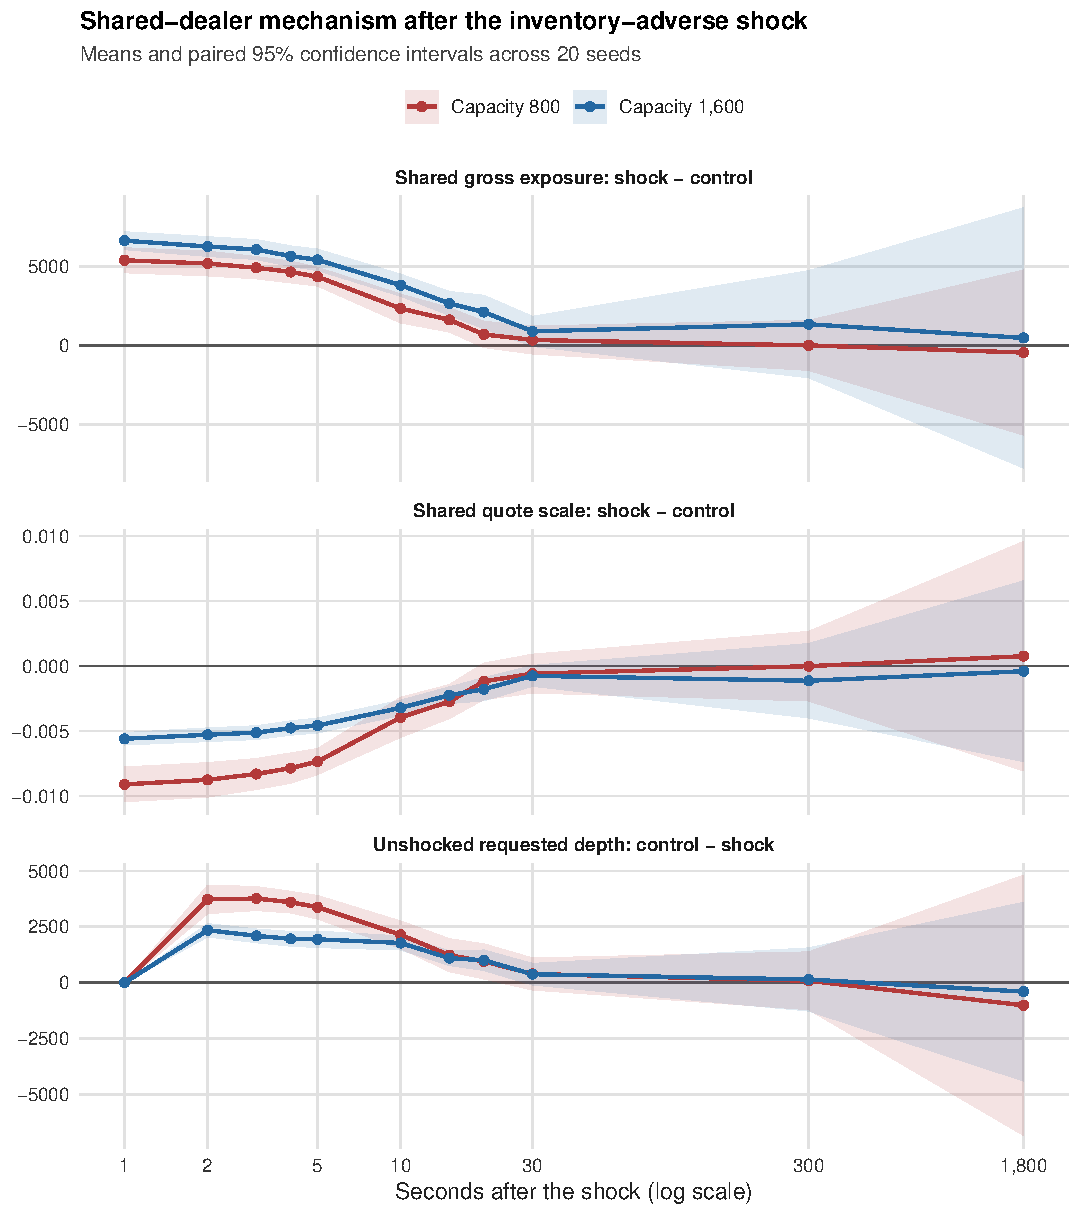
\includegraphics[width=0.83\textwidth]{docs/case-study/figures/mechanism_response.pdf}
\caption{Shared exposure, quote scale and requested depth after the shock.
Lines are seed means and shaded regions are paired 95\% confidence intervals.}
\label{fig:final_mechanism}
\end{figure}

\subsubsection{Market-wide liquidity response}

\begin{table}[htbp]
\centering
\caption{Liquidity response in unshocked books.  A positive depth value denotes
deterioration; brackets contain paired 95\% confidence intervals.}
\label{tab:final_liquidity}
\small
\begin{tabular}{rrrr}
\toprule
Horizon & $L$ & Relative top-depth change & Spread change (bp) \\
\midrule
2 s & 800   & $0.0568\%\ [0.0479,0.0656]$ & $0.00033\ [-0.00029,0.00094]$ \\
5 s & 800   & $0.0574\%\ [0.0462,0.0685]$ & $0.00135\ [-0.00176,0.00445]$ \\
5 s & 1,600 & $0.0420\%\ [0.0101,0.0738]$ & $0.00182\ [-0.00142,0.00505]$ \\
30-min mean & 800 & $0.1790\%\ [-0.2972,0.6552]$ & $-0.00115\ [-0.01431,0.01202]$ \\
30-min mean & 1,600 & $0.0108\%\ [-0.3815,0.4032]$ & $-0.00350\ [-0.01488,0.00787]$ \\
\bottomrule
\end{tabular}
\end{table}

The immediate response is statistically clear but economically small.
Top-of-book depth deteriorates by approximately 0.04--0.06\% during the first
few seconds (Table~\ref{tab:final_liquidity} and
Figure~\ref{fig:final_early_depth}).  The interval includes zero by
approximately 30 seconds.  No spread estimate in the main early or 30-minute
comparison is distinguishable from zero.  Moreover, the 30-minute depth
contrast between $L=800$ and $L=1{,}600$ is 0.168 percentage points with a
95\% confidence interval of $[-0.496,0.832]$.  The evidence therefore supports
a transient cross-asset withdrawal, but not a persistent liquidity spiral.

\begin{figure}[htbp]
\centering
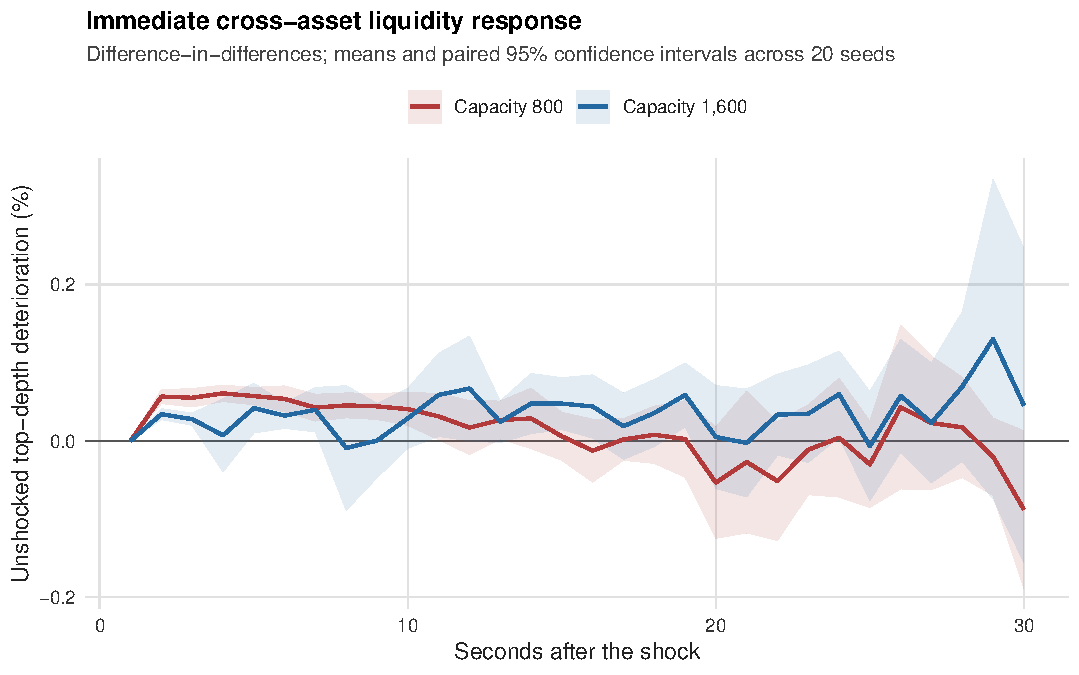
\includegraphics[width=0.83\textwidth]{docs/case-study/figures/marketwide_depth_early.pdf}
\caption{Difference-in-differences estimate of the immediate top-depth response
in unshocked books.}
\label{fig:final_early_depth}
\end{figure}

\subsubsection{Heterogeneity across liquidity clusters}

Cluster identifiers denote empirical categories and are not an ordinal
liquidity ranking.  Cluster sizes range from 70 to 266 books, so baseline depth,
spread and sample size must accompany any cluster label.  Averaged over seconds
2--10, nine of ten clusters at $L=800$ and eight of ten clusters at $L=1{,}600$
have positive depth effects whose paired intervals exclude zero.  The largest
estimates under $L=800$ occur in clusters 2 (0.157\%), 3 (0.132\%), 5
(0.124\%) and 0 (0.120\%).  The ordering is not monotone in baseline spread or
depth (Figure~\ref{fig:final_clusters}).

No cluster's 30-minute depth interval excludes zero under either capacity.
Two of 20 exploratory spread intervals exclude zero, but have opposite signs
and do not support a coherent result after accounting for multiple comparisons.
Thus the heterogeneous response is best interpreted as broad, short-lived
depth withdrawal rather than persistent cluster-specific contagion.

\begin{figure}[htbp]
\centering
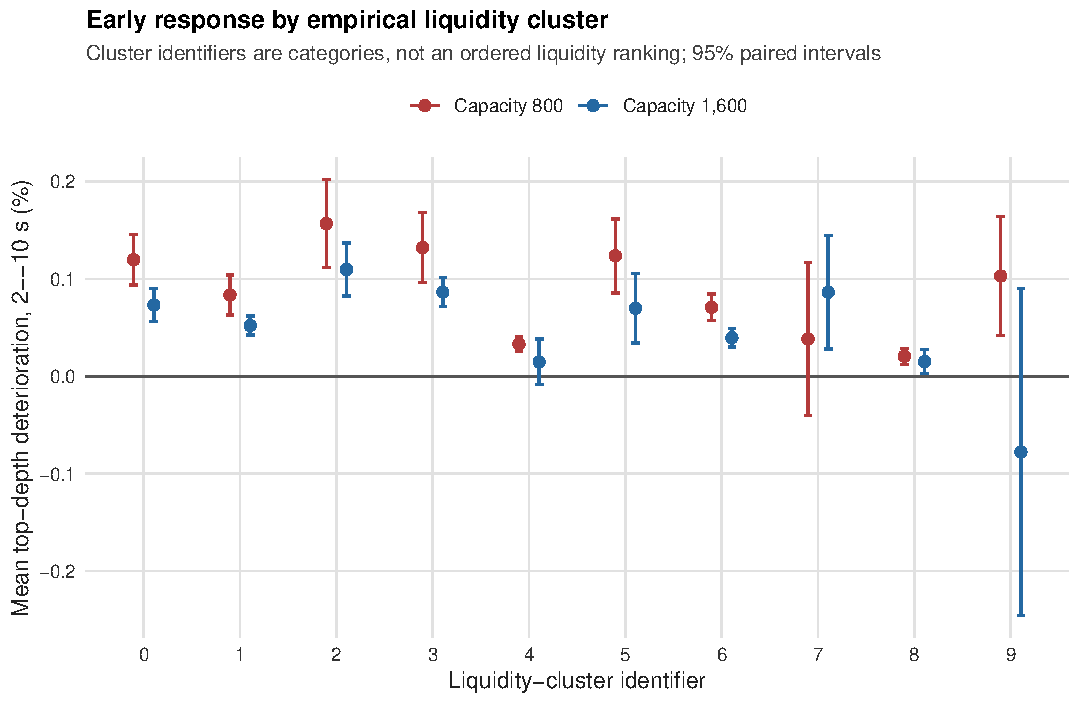
\includegraphics[width=0.83\textwidth]{docs/case-study/figures/cluster_early_response.pdf}
\caption{Mean top-depth deterioration during seconds 2--10 by empirical
liquidity cluster.  Error bars are paired 95\% confidence intervals.}
\label{fig:final_clusters}
\end{figure}

\subsubsection{Interpretation}

The experiment establishes that common inventory capacity can transmit an
adverse fill to otherwise unshocked books through a shared reduction in quoted
depth.  It also shows that the calibrated market replenishes this withdrawal
quickly.  The HPC contribution is integral to this inference: whole-book MPI
decomposition permits a deterministic, causally coupled 1,480-book
counterfactual matrix containing more than 25 billion processed orders.  The
result is evidence for a scalable and rank-independent mechanism experiment,
not historical replay or identification of an actual dealer's balance sheet.

